%% Problema: deve essere grassetto nella ToC e nel titolo del capitolo, ma non grassetto nell'header.
\chapter{\texorpdfstring{$\Lambda_b^0$}{Lambdab} and \texorpdfstring{$\Lambda^0$}{Lambda} decay vertex reconstruction}
\label{cap:vertex_reconstruction}

\section{Vertex reconstruction algorithms at LHCb}
\subsection{Vertex Fitter algorithm}
The Vertex Fitter (VF), implemented as part of the LoKi analysis toolkit, is the main vertexing algorithm used for the reconstruction of the $\Lambda_b^0$ decay.

Under VF formalism, each daughter particle is represented by a 7-dimensional vector
\begin{equation}
	\vec{p} = \begin{pmatrix}
		\vec{x} \\ \vec{q}
	\end{pmatrix}
	=
	\begin{pmatrix}
		x \\ y \\ z \\ p_x \\ p_y \\ p_z \\ E
	\end{pmatrix},
	\label{eq:particle_representation}
\end{equation}
combining the position $\vec{x}$ of the estimated origin vertex of the track (known as \textit{reference point}) with the 4-momentum $\vec{q}$ of the track constrained to originate in $\vec{x}$.
At the end of the fitting process, $\vec{x}$ will coincide with the common vertex chosen for all daughter particles.
Parameter vector \eqref{eq:particle_representation} has an associated covariance matrix $V$, which can be written in block structure as
\begin{equation}
	\begin{pmatrix}
		V_x      & V_{xp} \\
		V_{xp}^T & V_p
	\end{pmatrix}.
\end{equation}
It is also convenient to identify its formal inverse matrix $G := V^{-1}$, which has an analogous block form:
\begin{equation}
	\begin{pmatrix}
		G_x      & G_{xp} \\
		G_{xp}^T & G_p
	\end{pmatrix}
	=
	\begin{pmatrix}
		V_x      & V_{xp} \\
		V_{xp}^T & V_p
	\end{pmatrix}^{-1}
\end{equation}

The Vertex Fitter builds the decay tree from the bottom-up via a <<leaf-by-leaf>> approach, fitting one vertex at a time (e.g. $J/\psi \rightarrow \mu^+ \mu^-$, $\Lambda^0 \rightarrow p \pi^-$) and then moving upwards (e.g. $\Lambda_b^0 \rightarrow J/\psi \Lambda^0$).
This process is blind to the downstream leaves and only considers kinematic information of the immediate daughter particles, without accounting for momenta and mass constraints.

\subsubsection{Step}

The VF algorithm proceeds by \textit{steps}, with each step $k$ coinciding with the addition of the $k$-th daughter particle.

\begin{equation}
C_k^{-1} = C_{k-1}^{-1} + A_k^T G_k^B A_k
\end{equation}

\begin{equation}
E_k = -F_k C_k
\end{equation}

\begin{equation}
D_k = W_k - E_k F_k^T
\end{equation}

\begin{equation}
W_k = {\left(B_k^T G_k B_k\right)}^{-1}
\end{equation}

\begin{equation}
G_k^B = G_k - G_k B_k W_k B_k^T G_k
\end{equation}

\begin{equation}
F_k = W_k B_k^T G_k A_k
\end{equation}

\begin{equation}
\vec{x}_k = C_k \left[
	C_{k-1}^{-1} \vec{x}_{k-1}
	+
	A_k^T G_k^B \left(
		\vec{p_k} - c_k^0	
	\right)
\right]
\end{equation}

\begin{equation}
\vec{q}_k = W_k B_k^T G_k \left[
	\vec{p_k} - c_k^0 - A_k \vec{x}_k
\right]
\end{equation}

\begin{equation}
\begin{aligned}
\chi^2_k &= \chi^2_{k-1} \\
&+
\left[
	\vec{p} - c_k^0 - A_k \vec{x}_k - B_k\vec{q}_k
\right]^T G_k \left[
	\vec{p} - c_k^0 - A_k \vec{x}_k - B_k\vec{q}_k
\right] \\
&+
\left[
	\vec{x}_k - \vec{x}_{k-1}
\right] C_{k-1}^{-1} \left[
	\vec{x}_k - \vec{x}_{k-1}
\right]
\end{aligned}
\end{equation}

\begin{equation}
\vec{x}_k^n = \vec{x}_n
\end{equation}

\begin{equation}
\vec{q}_k^n = W_k B_k^T G_k \left[
	\vec{p}_k - A_k \vec{x}_n
\right]
\end{equation}

\begin{equation}
C_k^n = C_n
\end{equation}

\begin{equation}
D_k^n = W_k - E_k^n F_k^T
\end{equation}

\begin{equation}
E_k^n = - F_k C_n
\end{equation}

\begin{equation}
\text{corr}\left(
	\vec{q}_k^n, \vec{q}_l^n
\right) = F_k C_n F_l^T
\end{equation}

\begin{equation}
A_k = A = \begin{pmatrix}
1 \\
0
\end{pmatrix},
\quad\quad 
B_k = B = \begin{pmatrix}
0 \\
1
\end{pmatrix}
\end{equation}

\begin{equation}
G_k = \begin{pmatrix}
G_x 		&& G_{xp} \\
G^T_{xp} 	&& G_p
\end{pmatrix}
\end{equation}

\begin{equation}
W_k = G_p^{-1}
\end{equation}

\begin{equation}
G_k^B = \begin{pmatrix}
G_x - G_{xp}G_p^{-1}G_{xp}^T 	&& 0 \\
0								&& 0
\end{pmatrix}
\end{equation}

\begin{equation}
F_k = G_p^{-1} G_{xp}^T
\end{equation}

\begin{equation}
C_k^{-1} = C_{k-1}^{-1} + \left[
	G_x - G_{xp}G_p^{-1}G_{xp}^T
\right]
\end{equation}

\begin{equation}
E_k = -G_p^{-1} G_{xp}^T C_k
\end{equation}

\begin{equation}
D_k = G_p^{-1} + G_p^{-1} G_{xp}^T C_k G_{xp} G_p^{-1}
\end{equation}

\begin{equation}
\vec{x}_k = C_k \left[
	C_{k-1}^{-1} \vec{x}_{k-1}
	+ \begin{pmatrix}
		G_x - G_{xp} G_p^{-1} G_{xp}^T && 0
	\end{pmatrix}
	\left(
		\vec{p}_k - c_k^0
	\right)
\right]
\end{equation}

\begin{equation}
\vec{q}_k = \begin{pmatrix}
	G_p^{-1} G_{xp}^T && 0
\end{pmatrix}
\left[
	\vec{p_k} - c_k^0 - A\vec{x}_k
\right]
\end{equation}

\begin{equation}
\begin{pmatrix}
	G_x && G_{xp} \\
	G_{xp}^T && G_p
\end{pmatrix}
=
\begin{pmatrix}
	V_x && V_{xp} \\
	V_{xp}^T && V_p
\end{pmatrix}^{-1}
\end{equation}

\begin{subequations}
\begin{align}
&G_x - G_{xp} G_p^{-1} G_{xp} 	= V_x^{-1} \\
&G_p^{-1} 						= V_p - V_{xp}^T V_x^{-1} V_{xp} \\
&G_p^{-1} G_{xp}^T 				= -V_{xp}^T V_x^{-1}
\end{align}
\end{subequations}

When all particles have been added, i.e. all steps have been performed, the algorithm concludes an \textit{iteration}.
The process is then repeated until either a convergence condition is satisfied (see later) or the fit reaches the set number of allowed iterations, 10 by default.

\subsubsection{Seeding}

As one can observe, the procedure described above requires, at each step, both a previous estimated vertex position $\vec{x}_{k-1}$ and an associated inverse covariance matrix $C_{k-1}^{-1}$. In particular, step $k=1$ demands the existence of $\vec{x}_0$ and $C_{0}^{-1}$.

For iterations $i>1$, such roles are handily filled by the final vertex computed during the previous iteration. For the purpose of providing the first step of the first iteration with these values, at the beginning the algorithm tries to extract a \textit{vertex seed}, a first estimate of the decay vertex position, through a dedicated procedure depending on decay topology and properties of particles involved.

In the case of interest of the $\Lambda^0 \rightarrow p \pi^-$ two-body decay, said procedure is a simplified step of the Kalman filter:
\begin{subequations}
\begin{align}
	&C^{-1}_0 = {V_x}^{-1}_1 + {V_x}^{-1}_2 \\
	&\vec{x}_0 = C_0 \left(
		{V_x}^{-1}_1 \vec{x}_1 + {V_x}^{-1}_2 \vec{x}_2
	\right)
\end{align}
\end{subequations}
Subscripts $1$ and $2$ as used above refer to the two daughter particles in the decay (i.e. proton and pion).

\subsubsection{Termination and smoothing}


\subsection{Decay Tree Fitter algorithm}
[[@todo: Qui io darei una descrizione generale + FixJPsi + Lambda + reference, non serve per la discussione. Però ci starebbe un bel test in cui confronti la distribuzione dei vertici VF e DTF per mostrare che sono uguali (lo sono, vero??). Devi estrarli via Kinematic, immagino, perché nel rootfile non ci sono.]]

%% Con KineAtVtx non è più vero.
%For the purposes of the helicity angle analysis outlined in Section \ref{sec:lambda}, particle momenta computed with the DTF algorithm are particularly valuable because, in addition to their greater accuracy, they are provided directly at the production vertex;
%by contrast, VF momenta are provided either at the decay vertex (short-lived particles) or at the position of first measurement (long-lived or stable particles).

\section{Reconstruction efficiency of the \texorpdfstring{$\Lambda^0_b$}{Lambdab} and \texorpdfstring{$\Lambda^0$}{Lambda} decays}

To compute the vertex reconstruction efficiency for the $\Lambda_b^0$ decay chain, it is useful to conceptualize our event selection as a five step process:
\begin{enumerate}
	\item reconstruction of associated tracks for all charged daughter particles;
	\item reconstruction of the three decay vertices ($\Lambda^0$, $J/\psi$ and $\Lambda_b^0$);
	\item preliminary selections based on kinematic variables to filter out most background (see Section \ref{sec:prefilter});
	\item Decay Tree Fitter refit with appropriate mass constraints for the analysis at hand (usually $J/\psi$ and $\Lambda^0$);
	\item further selections applied to events passing all previous steps. Detailed in Chapter \ref{cap:event_selection}, these include a physical background veto and signal selection via a trained non-linear classifier.
\end{enumerate}

For the purposes of this section, we are interested in the first two steps (track and vertex reconstruction).

Efficiencies are computed with respect to \textit{reconstructible} particles, a flag attributed during the simulation process based on the number of \textit{hits} (charged clusters with defined positions) in specific modules of the LHCb detector.
A track is said to be reconstructible as VELO track with hits in $\geq 3$ VELO modules, while it's reconstructible as T track with $\geq 1$ hits in both the $x$ and stereo layers of each T station.
If these conditions are satisfied simultaneously, the track qualifies for reconstructibility as Long track \cite{Li:2752971}.

At Monte Carlo level, a track is deemed to be \textit{reconstructed} if it can be successfully matched to at least one MC particle;
for T and Long tracks, this is true if at least $70\%$ of the hits from the respective relevant detectors for reconstructibility are shared between reconstructed and true track. For $\Lambda^0_b$ events with a true $z_\text{vtx}^\Lambda \in [\SI{6.0}{\meter}, \SI{7.6}{\meter}]$, this results in a track reconstruction efficiency in the 60\% to 80\% range.

\begin{figure}[t!]
	\centering
	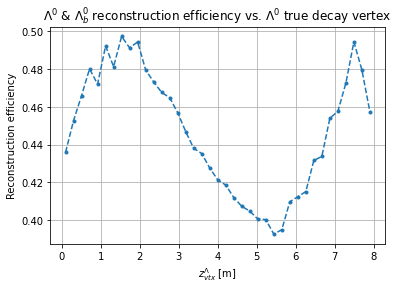
\includegraphics[width=.6\textwidth]{graphics/03-vertex_reconstruction/lambda_lambdab_reco_efficiency.png}
	\caption[A]{Reconstruction efficiency of simulated $\Lambda^0_b \rightarrow J/\psi~(\rightarrow \mu^+\mu^-)~\Lambda^0~(\rightarrow p\pi^-)$ events as function of the $z$ component of the true $\Lambda^0$ decay vertex. Assuming a $\approx 100\%$ reconstruction rate for the $J/\psi$ decay, the low efficiency is attributed to failure in reconstructing $\Lambda^0$ and $\Lambda^0_b$ decay vertices.}
	\label{fig:lambda_lambdab_reco_efficiency}
\end{figure}

When considering how many of these reconstructed charged particles pass the vertex reconstruction (\textit{vertexing}) process, the computed efficiency is much lower.
Figure \ref{fig:lambda_lambdab_reco_efficiency} plots the resulting $\Lambda_b^0$ vertexing efficiency through the whole true $z_\text{vtx}^\Lambda$ spectrum, showing that said efficiency never manages to get past the 50\% threshold.
This means that over half of our candidate signal events is lost during the second step of the five step selection process.

While available information does not distinguish between the three individual vertexing phases ($J/\psi$, $\Lambda^0$ and $\Lambda_b^0$), we can make some reasonable assumptions.
Being Long tracks, muons and antimuons have well reconstructed momentum with constraints across the LHCb detector;
for this reason their influence on the vertexing efficiency dip is considered negligible.
Furthermore, the rare usage of T tracks for physics analysis in LHCb suggests that problems are likelier to arise in the $\Lambda^0 \rightarrow p\pi^-$ vertexing and then cascade into the $\Lambda_b^0 \rightarrow J/\psi~\Lambda^0$ reconstruction.

For the above reasons, in the following sections I'll focus on the $\Lambda^0$ decay to search for issues and solutions, with the goal of improving our signal statistic. %% O statistics?


\section{Characterization of non-converged events}
Qui devi dire: protone momento basso in z, interpolateOnlyLongTracks, ...

\section{Uncertainty-based algorithms for the recovery of non-converged events}
